\documentclass[anonymous,12pt]{iopjournal}
\usepackage{amsmath,amssymb,amsthm,booktabs,array,microtype,graphicx,placeins}
\graphicspath{{figures/}}
\hypersetup{hidelinks,pdftitle={Lower bounds on peak dielectric contrast from finite-aperture scattering data},pdfauthor={},pdfsubject={Inverse electromagnetic scattering}}
\fancyhead[L]{\small\sffamily Inverse Problems\quad Research paper}
\fancyhead[R]{\small Peak contrast from scattering data}
\newtheorem{theorem}{Theorem}[section]
\newtheorem{proposition}[theorem]{Proposition}
\newtheorem{lemma}[theorem]{Lemma}
\newcommand{\C}{\mathbb C}\newcommand{\R}{\mathbb R}
\newcommand{\Herm}{\operatorname{Re}_{H}}\newcommand{\Imag}{\operatorname{Im}_{H}}
\newcommand{\tr}{\operatorname{tr}}\newcommand{\diag}{\operatorname{diag}}
\newcommand{\dist}{\operatorname{dist}}\newcommand{\rank}{\operatorname{rank}}\newcommand{\ran}{\operatorname{ran}}
\newcommand{\norm}[1]{\left\|#1\right\|}\newcommand{\dd}{\mathrm d}
\newcommand{\Dpos}{D_{\mu}}\newcommand{\Dopt}{D_{\lambda}}
\numberwithin{equation}{section}
\setlength{\headheight}{17pt}\setlength{\emergencystretch}{1.7em}
\setcounter{topnumber}{3}\setcounter{bottomnumber}{2}
\renewcommand{\topfraction}{.91}\renewcommand{\textfraction}{.07}
\begin{document}
\noindent{\sffamily\small RESEARCH PAPER}\par\vspace{1.8ex}
\title{Lower bounds on peak dielectric contrast from finite-aperture scattering data}
\author{}
\begin{abstract}
Can a microwave array establish that a dielectric exceeds a given contrast somewhere, before forming an image? An unobserved current may carry power away from a partial aperture. Different incident fields, however, must drive currents in the same material. We combine these restrictions to bound the distance from the complex measurements to every medium below a given peak. The number of negative directions of a weighted current operator determines how many eigenvalues can be lost from a measured illumination spectrum. We construct examples in which each coherent illumination admits an exact receiver fit under four regional power balances and a physical current-energy bound, yet the joint data rule out the contrast range. Sixteen regional balances recover the same exclusion for a single coherent combination. In a 9,216-cell transverse-magnetic model at 400 MHz and 2\% noise, increasing the number of incident directions from ten to twenty-four at fixed total fluence establishes peak contrast above 0.75 on five of six objects, up from two. Moving to thirty-two directions changes none of these outcomes. Their negative current directions are almost entirely invisible to the receivers and have large outgoing wave-equation defects in the uniform capped medium. A separate port weighting rules out every nonnegative first-Born image on the same six objects. A near-noise reconstruction and measurements from two microwave chambers delimit what the bounds establish about material recovery and model error.
\end{abstract}
\keywords{electromagnetic inverse scattering, optical theorem, dielectric contrast, illumination diversity, finite aperture, uncertainty bounds}

\section{Introduction}
A smooth, low-contrast image may predict a measured scattered field within a few noise radii. Is the small discrepancy a consequence of a misplaced inclusion, or would \emph{every} arrangement of material at that contrast miss the data? These alternatives suggest different actions. The first calls for refining the image. The second gives a reason to increase the permitted contrast before spending another forward solve. We study this second question at one frequency, with an arbitrary nonnegative contrast at every cell in a two-dimensional dielectric.

A receiver measures only a projection of the contrast current. The remaining current is precisely the difficulty exploited by the subspace optimization methods of Chen and of Zhong and Chen \cite{chen,zhong,ffttsom}. An array restricted to half a circle can miss currents that radiate substantial power in other directions. Conversely, a sufficiently dense full circle can account for nearly all radiated power and still leave many interior currents unobserved. A second physical restriction survives either layout. Although the currents change with the illumination, their ratio to the total electric field at each point must describe the same dielectric. This relation couples illuminations even when each individual reading admits a current consistent with conservation of power.

Our main result gives a lower bound in the units measured by the array. For a proposed peak contrast, form a Hermitian matrix on currents and a much smaller matrix on illuminations. If the former has four negative directions, at most the first four eigenvalues of the latter can be lost. A positive remainder above the squared noise radius excludes the entire contrast range. We exhibit two observations for which a single usable coherent combination exists for a sufficiently fine spatial partition, whereas every single coherent test with four regions attains zero residual, even with a physical current-energy limit. All comparisons use the same array and the same noise ball. The difference is in which restrictions on a common set of currents can be enforced.

The approach builds on several results with different inverse or design objectives. Bounds on photonic design performance and on scattered fields follow from the wave equation and power conservation \cite{angeris19,trivedi,angeris}. Real and reactive power constraints, their spatial subdivisions and cross-excitation terms have been used for electromagnetic design \cite{moleskyglobal,moleskylocal,kuang,shim}. Tian gives extremal-inertia formulas for matrix quadratics \cite{tian}. Continuous inverse scattering also uses operator inequalities modulo finitely many negative directions to obtain support information \cite{griesmaier_harrach,griesmaier_harrach_erratum,albicker}. Here the two conclusions are obtained for the same incomplete data: feasibility of each coherent receiver reading under explicit regional relaxations, and a positive distance from the \emph{joint} reading to all physical media below a stated peak. Neither conclusion requires an initial reconstruction.

The implications for imaging depend on the angular information actually present. Following the spatial-bandwidth analysis of Bucci and Franceschetti \cite{bucci87,bucci89}, we vary both arrays at fixed incident fluence and compare independently computed angular responses. We also test the linear first-Born model directly. Ruling out a low peak in the nonlinear equations alone does not answer the Born question, because a linear inversion is free to use a larger contrast. Finally, we compare the material images obtained when the contrast range is enlarged under different stopping rules.

\section{A lower bound from the current and the measured field}\label{sec:joint}

\subsection{Outgoing transverse-magnetic scattering}
Take the time dependence $\exp(-\mathrm i\omega t)$, a nonmagnetic medium invariant in the axial direction, and an axial electric field. In a homogeneous background of wavenumber $k$ let $\chi$ be the relative dielectric contrast and $\Omega$ the part of the transverse plane in which it may vary. Put $j=\chi E$, where $E$ denotes the total electric field. The outgoing Green function is $\Phi_k(x)=\mathrm i H_0^{(1)}(k|x|)/4$. For one incident field $b$,
\begin{equation}
 (\Delta+k^2)E=-k^2j,\qquad
 E(x)=b(x)+k^2\int_\Omega\Phi_k(x-x')j(x')\,\dd x'. \label{eq:wave}
\end{equation}
The measured scattered field is the integral term evaluated at the receivers. This is the volume-integral formulation of dielectric scattering \cite{colton,chenbook}.

On a square pulse grid of side $h$, the principal synthetic experiment integrates each source cell as an equal-area disk of radius $\rho=h/\sqrt{\pi}$ and collocates at the cell centres $x_i$ \cite{richmond}. With $q=k\rho$ and $c_q=\pi qJ_1(q)/2$, the resulting entries are
\begin{equation}
 G_{ij}=\mathrm i c_qH_0^{(1)}(k|x_i-x_j|)\quad(i\ne j),
 \qquad G_{ii}=\mathrm i\pi q H_1^{(1)}(q)/2-1. \label{eq:disk}
\end{equation}
Replacing the observation centre in the off-diagonal formula by an exterior receiver gives $S_{\ell j}$. The incident columns for the full-ring experiment are
$B_{ij}=\sqrt{10/s}\,\exp(\mathrm ik\,\widehat d_j\cdot x_i)$.
Each receive row carries the factor $\sqrt{20/p}$ for angular quadrature. Ten unit-amplitude shots and the denser arrays therefore have the same total incident fluence per unit reference aperture. The angular comparison has no implicit assumption about absolute transmitter watts. Cylindrical transmitters use the outgoing Hankel field and the stated chamber calibration. Table~\ref{tab:electrical-acquisitions} gives the physical dimensions and port counts for each experiment.

Collect $s$ incident fields in $B$, $s$ total fields in $E$ and the corresponding currents in $J$. If $X=\diag(\chi_i)$, the full and linear data maps are respectively
\begin{equation}
 E=B+GJ,\quad J=XE,\quad F(\chi)=SJ,\qquad F_{\rm B}(\chi)=SXB .
 \label{eq:vie}
\end{equation}
For a complex square matrix $T$ write $\Herm T=(T+T^*)/2$, $\Imag T=(T-T^*)/(2\mathrm i)$. The Hermitian radiation part $R=\Imag G$ has entries $c_q J_0(k|x_i-x_j|)$, including the diagonal. Their plane-wave angular integral gives
\begin{equation}
 j^*Rj=\frac{c_q}{2\pi}\int_0^{2\pi}
 \left|\sum_i j_i\exp(-\mathrm i k\widehat d_\theta\cdot x_i)\right|^2\dd\theta .
 \label{eq:power}
\end{equation}
The outgoing sign and the positive $c_q$ for the cell sizes used here give nonnegative radiated power. The continuous kernel has the analogous Gram representation. A stored rounded matrix is treated in its own arithmetic when a strict inequality is asserted. The physical forward map includes all orders of multiple scattering on its declared grid.

\subsection{Common material and the residual left across illuminations}
Let $Y$ denote the measured complex field and $r$ its joint error radius. We test all $0\le X\le U=\diag(u_i)$. For nonnegative real diagonal $D_\mu$ and real diagonal $D_\lambda$, each physical current satisfies
\begin{align}
 Q_{\rm r}&=J^*D_\mu J-\Herm(J^*D_\mu U E)
       =E^*D_\mu X(X-U)E\preceq0,\nonumber\\
 Q_{\rm o}&=\Imag(J^*D_\lambda E)=0 .\label{eq:balance}
\end{align}
Each diagonal entry involves a single incident field. The off-diagonal entries impose the same law on every coherent linear combination of incident fields. For passive complex contrast, the same argument gives $Q_{\rm o}\preceq0$ when $D_\lambda\succeq0$, and $Q_{\rm r}\preceq0$ when $|\chi_i|^2\le u_i\Re\chi_i$. This disk in the complex contrast plane specifies the loss convention used below.

\begin{proposition}[Shared material at one cell]\label{prop:pixel}
For actual currents, enforcing both balances separately at each cell is equivalent to the existence of a common real $0\le X\le U$ satisfying \eqref{eq:vie}.
\end{proposition}
\begin{proof}
Write $j_i,e_i$ for the rows of $J,E$. On $\ker e_i$ the sector inequality reduces to $|j_i a|^2\le0$. Thus $j_i$ vanishes when $e_i=0$. Otherwise $j_i=\alpha_i e_i$ for some complex $\alpha_i$. The optical equality makes $\alpha_i$ real and the sector inequality gives $\alpha_i(\alpha_i-u_i)\le0$. The converse follows by substitution. Summing cell inequalities yields the regional laws, and summing children gives the law of a parent region. The first assertion applies to rank-one current moments when a lift is used.
\end{proof}

Set $Z=(D_\mu U+\mathrm iD_\lambda)/2$ and define
\begin{align}
 K&=S^*S+D_\mu-ZG-G^*Z^*,\qquad L=S^*Y+ZB,\nonumber\\
 H_Y&=Y^*Y-L^*K^{-1}L .\label{eq:operators}
\end{align}
The current matrix $K$ depends on the array, propagation and material hypothesis. The source matrix $H_Y$ additionally depends on the actual measured field.

\begin{theorem}[A joint lower distance]\label{th:bound}
Suppose $K$ is nonsingular and let $\nu=n_-(K)$. Write $h_1\ge\cdots\ge h_s$ for the eigenvalues of $H_Y$. For every physical current obeying \eqref{eq:balance},
\begin{equation}
 \norm{SJ-Y}_F^2\ \ge\ d^2=\sum_{j=\nu+1}^s(h_j)_+,\qquad
 (x)_+=\max(x,0).\label{eq:bound}
\end{equation}
If $d>r$ and $U=uI$, every material compatible with the readings has peak contrast exceeding $u$. The weights may be chosen from the data.
\end{theorem}
\begin{proof}
Put $D=(SJ-Y)^*(SJ-Y)\succeq0$. Add \eqref{eq:balance} to obtain
\begin{equation}
 D\succeq H_Y+(J-K^{-1}L)^*K(J-K^{-1}L).\label{eq:completion}
\end{equation}
The negative part of the last quadratic has rank at most $\nu$. Rank interlacing gives $\lambda_i(D)\ge h_{i+\nu}$ for $i+\nu\le s$. Taking the nonnegative part and summing proves the result. The value is sharp if the only remaining information is $D\succeq0$ and $D\succeq H_Y+T^*KT$ with $T$ free: $\nu$ rescaled negative directions of $K$ cancel up to the first $\nu$ positive eigenvalues. This statement of sharpness pertains to the relaxed trace problem.
\end{proof}

A singular $K$ can also give a bound. For $\alpha\ge0$ set
$\mathcal P_\alpha=\left(\begin{smallmatrix}K&-L\\-L^*&Y^*Y-\alpha I_s\end{smallmatrix}\right)$.
If $\mathcal P_\alpha$ has $n+b$ positive eigenvalues, its restriction to the $s$-dimensional graph $[J;I_s]$ has at least $b$ positive directions by dimension counting. Since $D-\alpha I_s$ bounds this restriction from above, at least $b$ eigenvalues of $D$ exceed $\alpha$. Integrating the resulting count in $\alpha$ bounds $\tr D$, as can a finite lower sum. Related extremal-inertia identities are given in \cite{tian}.

For incomplete acquisition, disjoint source groups may retain their respective common receiver rows. Distances $d_g$ then combine in quadrature across disjoint entries. For a unit coherent vector $a$, the same joint ball implies $\|(Y-F)a\|\le r$. These are comparisons of the same exposures. To transfer an ideal-model result, suppose
$Y=(I+T)(F(\chi)+b_{\rm mod})+n_{\rm add}$, with
$\norm{T}\le\eta<1$, $\norm{b_{\rm mod}}_F\le b$ and $\norm{n_{\rm add}}_F\le\delta$. A sufficient radius, in the measured units, is
\begin{equation}
 r_{\rm eff}=b+\frac{\delta+\eta\norm{Y}_F}{1-\eta}.
 \label{eq:budget}
\end{equation}
This follows by inverting $I+T$ in the vectorized measurement space. Repeated use of the same gain must respect its common value. A calibration residual gives an empirical scale, whereas a physical material inference requires an error budget that covers the loaded target.

\section{Radiated power, coherent illumination and electrical size}\label{sec:single}

\subsection{Power outside the measured aperture}
Let $\Pi_0$ project orthogonally onto $\ker S$, put $H=\Herm G$ and let $R_0=\Pi_0R\Pi_0$. For spatially constant weights $D_\mu=\mu I$, $D_\lambda=\mu tI$ and a uniform hypothetical cap $u$, every receiver-invisible current $w$ satisfies
\begin{equation}
 w^*(K/\mu)w=\|w\|^2-u\,w^*Hw+t\,w^*Rw .\label{eq:dark}
\end{equation}
On a half circle a current can have $Sw=0$ while radiating strongly outside the measured arc. Increasing $t$ then increases its cost. If $R_0$ is very small even a large optical weight can have little effect. The first hidden loss of positivity for $t\ge0$, when $R_0\succeq0$, is
\begin{equation}
 u_*(t)=\inf_{\substack{Sw=0\\w^*Hw>0}}
    \frac{\|w\|^2+t\,w^*Rw}{w^*Hw}.
\end{equation}
It is nondecreasing and concave on its finite domain as an infimum of affine functions. A positive lower eigenvalue $\alpha$ of $R$ restricted to the receiver kernel gives a slope at least $\alpha/\|H\|_2$. There need be no useful uniform lower slope on refining the grid. A practical upper estimate of hidden radiated power follows from
\begin{equation}
 \|R_0\|_2\le\|R-S^*T-T^*S\|_F\qquad\text{for every }T\in\C^{p\times n}.
 \label{eq:radupper}
\end{equation}
Compression to $\ker S$ removes the last two terms. A positive Rayleigh quotient of an actual hidden current supplies the complementary lower estimate.

\subsection{The same physical measurements as one coherent input}
For unit $a\in\C^s$, set $b=Ba$ and $y_a=Ya$. The global sector and optical balances for a single current read
\[
 q_r(j)=j^*(I-uH)j-u\Re(j^*b),\qquad
 q_o(j)=j^*Rj+\Im(j^*b).
\]
A coherent fit requires $Sj=y_a$, $q_r(j)\le0$ and $q_o(j)=0$. It allows a distinct fit for each choice of incident field. A common physical material must satisfy the matrix balances for a single current matrix across all fields.

\begin{theorem}[Separate coherent fits and joint exclusion]\label{th:two}
Suppose $w\in\ker S$ has $\rho_w=w^*Rw>0$ and
$w^*(I-uH)w+t_0\rho_w<0$. Suppose a matrix $C_0$ with $SC_0=Y$ has, for every unit $a$ and $x=C_0a$,
$q_o(x)<0$ and $q_r(x)+t_0q_o(x)<0$.
Each coherent input admits a current $j_a$ attaining zero receiver residual and both global constraints with strict sector slack. If \eqref{eq:bound} exceeds the noise level, the joint data exclude the same peak hypothesis.
\end{theorem}
\begin{proof}
Choose $|\beta|^2=-q_o(x)/\rho_w$. The cross term in $q_o(x+\beta w)$ is a real linear function of the phase coordinates of $\beta$ and can be made zero. Either sign of that phase then yields $q_o=0$. Select the sign giving a nonpositive sector cross term. The sector value is at most
$q_r(x)+t_0 q_o(x)+|\beta|^2w^*(I-uH+t_0R)w<0$. Since $Sw=0$, the receivers see $y_a$ in each case.
\end{proof}
The lifted single-source problem minimizes squared receiver residual subject to positive semidefinite moments, the two global balances and unit homogeneous coordinate. These same hypotheses give a strict Slater point relative to the optical equality. Keep mean $x$ and assign current covariance
$\varepsilon I+c_\varepsilon ww^*$ with
$c_\varepsilon=(-q_o(x)-\varepsilon\tr R)/\rho_w$.
For small $\varepsilon>0$ the covariance is positive definite, the optical equality holds, and the sector remains negative by continuity. The residual is $\varepsilon\|S\|_F^2$. The exact rank-one fit already attains zero. Thus the primal and dual optima are zero under simultaneous global constraints, including the limiting dual weights \cite{boyd,beck}.

For a partition with cell indicators $D_b$, take receiver-invisible vectors $w_j$ and set
\[
 k_{bj}=w_j^*D_bw_j-u\Re(w_j^*D_bGw_j),\quad
 l_{bj}=\Im(w_j^*D_bGw_j).
\]
Let $Q_{r,b}(C_0),Q_{o,b}(C_0)$ be the two source balances on a region for the receiver fit $C_0$. Sufficient conditions for zero optimal lifted distance, for \emph{all} unit $a$, are the existence of $P_j\succeq0$ with
\begin{equation}
 Q_{r,b}(C_0)+\sum_j k_{bj}P_j\preceq0,\qquad
 Q_{o,b}(C_0)+\sum_j l_{bj}P_j=0 .\label{eq:regionalmoment}
\end{equation}
Indeed the mean $C_0a$ and covariance $\sum_j(a^*P_j a)w_jw_j^*$ have exactly these moments and zero receiver variance. They also satisfy a physical energy cap $\mathcal P$ whenever
$C_0^*C_0+\sum_j\|w_j\|^2P_j\preceq\mathcal P I_s$.
For the opposite comparison, when $K\succ0$, the best single coherent input for the given weights has squared lower bound $(h_1)_+$. It equals the joint bound whenever only one source eigenvalue is positive. These two constructions permit an exact comparison with spatially resolved single-source models.

\subsection{Increasing the angular sampling}
The receiver geometry affects $\nu$, while the incident angular bandwidth affects the field left after the first $\nu$ terms have been removed. For scalar weights let $A_t=I+tR+S^*S/\mu$. If $A_t\succ0$ and $u>0$, then
\[
 n_-(K)=\#\{\lambda(A_t^{-1/2}H A_t^{-1/2})>1/u\}.
\]
Adding the positive receiver term can remove at most $\rank S$ negative directions at fixed $t$. For comparison, a periodic Helmholtz convolution away from a lattice pole has reactive symbol $k^2/(|\xi|^2-k^2)$. The annulus $k<|\xi|<k\sqrt{1+u}$ then contributes negative directions of $I-uH$ and has an area corresponding to roughly $|\Omega|k^2u/(4\pi)$ lattice points. This comparison motivates an electrical-area scale. For the open, bounded scatterer we calculate the actual inertia. A negative direction of $K$ need not solve a homogeneous Maxwell equation.

The incident direction has its own scale. Let $A$ be the active cells of a particular medium, $a_A$ the radius of a disk containing them, and $T_A=(I-X_A G_{AA})^{-1}X_A$ on a regular forward solution. At fixed material the measured response is linear in the incident plane wave restricted to $A$. Its angular Fourier coefficient $f_\ell$ obeys
\begin{equation}
 \|f_\ell\|_2\le
 \|S_AT_A\|_2\Big(\sum_{i\in A}|J_\ell(k|x_i|)|^2\Big)^{1/2}.
 \label{eq:bandwidth}
\end{equation}
Here the transmit amplitude is one and the origin is taken at the enclosing disk centre. Equation~\eqref{eq:bandwidth} follows by the Jacobi--Anger expansion at each cell and includes all orders of multiple scattering in $T_A$. The Bessel tail decays rapidly beyond $ka_A$. The usual angular count of order $2ka$ is therefore tolerance dependent \cite{bucci87,bucci89}. The search domain has a known enclosing radius before inversion. The actual supports, used only to interpret measured interpolation errors, can be much smaller.

There is an exact limiting control. If a right multiplication by $V$ with $VV^*=I_s$ duplicates or mixes the columns of both $B$ and $Y$, the new source form is $V^*H_YV$ and the total incident fluence is preserved. Its positive eigenvalues and the bound are unchanged. For approximate redundancy, for any source-space orthogonal projection $P$ of codimension at most $\nu$, interlacing under compression gives
\begin{equation}
 d^2\le\tr[(PH_YP)_+]\le
 \|YP\|_F^2+\|(-K^{-1})_+^{1/2}LP\|_F^2 .\label{eq:tail}
\end{equation}
For the second inequality drop the nonpositive contribution from the positive spectral space of $K^{-1}$, leaving a positive semidefinite upper matrix. This shows explicitly why $s>\nu$ gives an opportunity for exclusion and still permits a vanishing or very small bound.

\section{Evaluation on the full material grid}\label{sec:fourier}

\subsection{A one-sided Fourier bound}
Zero padding and the unitary discrete Fourier transform define an isometry $V_F$. On a rectangular grid the stored volume operator has the form $G=V_F^*\diag(g_q)V_F$. For spatially uniform weights let $\sigma_q=1-u\Re g_q+t\Im g_q$. Choose a subset $\mathcal I$ of frequencies and a floor $f\le\min_{q\notin\mathcal I}\sigma_q$. Then
\begin{equation}
 K\succeq S^*S+\mu f I+
     \mu\sum_{q\in\mathcal I}(\sigma_q-f)\,v_qv_q^*,\qquad v_q=V_F^*e_q .
 \label{eq:floor}
\end{equation}
The omitted terms are bounded on \emph{all} cell currents. A positive diagonal floor plus a signed low-rank update reduces the inertia calculation. For $A_0+WCW^*$ with $A_0\succ0$, $C$ Hermitian invertible and its reduced Schur complement nonsingular, block elimination gives
\[
 n_-(A_0+WCW^*)=n_+(C^{-1}+W^*A_0^{-1}W)-n_+(C^{-1}).
\]
For $25^2$ selected modes and 20 receivers the reduced order is 645, while all 9,216 cell values remain independent. Regional weights require both $V_F j$ and the Fourier transform of a spatially weighted current, as detailed in Appendix~\ref{app:replay}. Trial subspace construction, evaluation of neglected modes and unsuccessful gap searches contribute to the actual computation.

To evaluate the source form on the original grid, put $A_K=K/\mu$, $L_K=L/\mu$ and let $C_1$ approximate $A_K^{-1}L_K$. With $\Delta=A_K C_1-L_K$,
\begin{equation}
 H_Y=Y^*Y+\mu(C_1^*A_KC_1-C_1^*L_K-L_K^*C_1)-\mu\Delta^*A_K^{-1}\Delta .
 \label{eq:native}
\end{equation}
A lower bound $g>0$ on every positive eigenvalue of $A_K$ makes the correction bounded from below by $-\mu\|\Delta\|_2^2 I/g$. The negative index is checked separately. Positive regions of the remaining source spectrum give a distance in the same field units as the observations. A new data matrix on a fixed array reuses the state calculation.

For a spatial indicator $D_b$ and uniform cap $u$, put $J_0=K^{-1}L$ and $E_0=B+GJ_0$. On a smooth interval of weights with fixed $\nu$, let $P_+$ project onto the retained positive source eigenvalues. The derivatives of $d^2$ are the traces against $P_+$ of $J_0^*D_bJ_0-u\Herm(J_0^*D_b E_0)$ and $\Imag(J_0^*D_b E_0)$ for sector and optical weights respectively. Stationarity cancels the derivative of $J_0$. Only clusters separated at zero and at the removal index admit this expression. Regional searches can use the derivatives and then evaluate \eqref{eq:native} at the chosen weights.

\subsection{A direct test of the first-Born model}
The nonlinear box in Theorem~\ref{th:bound} and the linear model $F_{\rm B}$ in \eqref{eq:vie} have different feasible fields. Let $\langle A,B\rangle_F=\tr(A^*B)$. For any array weight $Z_{\rm B}\ne0$, put $g_i=\Re\langle Z_{\rm B},S_{\cdot i}B_{i\cdot}\rangle_F$. Convex separation and Cauchy--Schwarz give
\begin{equation}
 \dist_{\rm B}(Y,[0,U])\ \ge\
 \frac{\big(\Re\langle Z_{\rm B},Y\rangle_F-\sum_i u_i(g_i)_+\big)_+}{\|Z_{\rm B}\|_F}.
 \label{eq:born}
\end{equation}
Here $\dist_{\rm B}$ is the distance to all corresponding Born fields. When $g_i\le0$ throughout, the sum vanishes, even for the entire unbounded nonnegative material cone.

A useful direction comes directly from extinction. Fit $S^*C\approx B$ by truncated least squares and set $q_i=\sum_j(S^*C)_{ij}\overline{B_{ij}}$. If all real parts are positive, take
$\eta_{\rm B}\ge\max(0,\max_i-\Im q_i/\Re q_i)$ and $Z_{\rm B}=(\mathrm i-\eta_{\rm B})C$.
Then $g_i=-\Im q_i-\eta_{\rm B}\Re q_i\le0$. If the receiver can match $S^*C=B$ exactly and $\eta_{\rm B}=0$, the signed reading on physical currents is
$\Im\tr(B^*J)=\tr(J^*RJ)$ by the lossless optical identity. For a real Born current it vanishes. For a finite, masked array the inequality uses the signs of the actual cell pairings. The fit need only produce the required signs. With different masks by source, each column uses its actual receivers and its cell pairing contributes to the same real sum. This specialization of ordinary cone separation needs only one complex inner product for a new target on the same array.

\paragraph{Implementation and validation.}
Codex (OpenAI) was used to develop and execute the Fourier, full-wave and bounded-inversion calculations. Gemini (Google) was used to examine the acquisition operators and to suggest controls for angular sampling and illumination redundancy. The numerical checks compare full-wave fields at independently sampled angles, enclose the state and source spectra on the original grid, and evaluate reconstructed maps on withheld ports. Generating materials are used for simulation, feasibility checks and offline scoring. They are withheld from the bounds and inversion routines. All physical figures are drawn from the saved arrays.

\section{Numerical experiments}\label{sec:exp}

\subsection{Radiation with half-ring and full-ring reception}\label{sec:exp-radiation}

Table~\ref{tab:electrical-acquisitions} gives the electrical size of each experiment. For a square of width \(W\), we use the circumscribed radius \(a=W/\sqrt{2}\). The main synthetic experiment uses six lossless distributions on a \(96^2\) grid at \(400\,\mathrm{MHz}\), with wave speed \(3\times10^8\,\mathrm{m\,s^{-1}}\). The original arrays have ten unit-amplitude plane waves and twenty receivers at radius \(3.75\,\mathrm{m}\). Changing the aperture changes both the illumination and receiver angles. The numerical model is the scalar TM volume integral equation on the indicated grid throughout. Each synthetic noise radius is the realized Frobenius noise norm plus \(10^{-6}\|Y\|_F\), with the latter allowance covering the error of the finite-dimensional generating solve. Unless stated otherwise, a rigorous lower bound comes from outward rounding on the original grid. Area averaging the same six contrast maps to \(32^2\) and solving there changes the synthetic fields by 12.4--28.4\% on the half ring and 14.2--35.4\% on the full ring. These are differences at the reference maps. The bounds below use all \(9{,}216\) native cells.

\begin{table}[tbp]
\centering\small
\caption{Electrical dimensions and material ranges. The Manitoba rows give the frequency endpoints. Receivers are counted per illumination. In Manitoba each of two complementary groups has 12 transmitters and 12 receivers. In Fresnel the permitted receivers change with the source. The annular benchmark specifies dimensions in wavelengths. Chamber contrasts are nominal.}
\label{tab:electrical-acquisitions}
\setlength{\tabcolsep}{3.15pt}
\begin{tabular}{@{}lrrrrrrll@{}}
\toprule
Experiment & Grid & GHz & \(W\) (m) & \(W/\lambda\) & \(ka\) & \(2ka\) & \(s,p\) & Contrast\\
\midrule
Annular inclusion & \(24^2\) & -- & -- & 0.96 & 4.27 & 8.53 & \(12,48\) & \(0.1\)--\(12\)\\
Austria & \(32^2\) & 0.4 & 2 & 2.67 & 11.85 & 23.70 & \(20,40\) & \(0\)--\(3\)\\
Six shapes & \(96^2\) & 0.4 & 2 & 2.67 & 11.85 & 23.70 & \(10\)--\(32,20/32\) & \(0\)--\(3.63\)\\
Compact patch & \(12^2\) & 0.4 & 0.125 & 0.167 & 0.740 & 1.481 & \(10,20\) & \(0\)--\(0.879\)\\
Manitoba & \(40^2\) & 3 & 0.14 & 1.40 & 6.22 & 12.45 & \(12,12\) & \(1.30,\ 2.03+0.03\mathrm{i}\)\\
 & \(40^2\) & 6 & 0.14 & 2.80 & 12.45 & 24.90 & \(12,12\) & same\\
Fresnel & \(60^2\) & 4 & 0.20 & 2.67 & 11.86 & 23.71 & \(8/18,241\) & \(0,\ 0.45,\ 2\)\\
 & \(60^2\) & 6 & 0.20 & 4.00 & 17.78 & 35.57 & \(8/18,241\) & same\\
 & \(60^2\) & 8 & 0.20 & 5.34 & 23.71 & 47.42 & \(8/18,241\) & same\\
\bottomrule
\end{tabular}
\end{table}

A current in \(\ker S\) can radiate between receivers. Equation~\eqref{eq:radupper} controls the radiation retained in this space. On the \(96^2\) grid, \(\|R\|_2\simeq5.095\), whereas the leading numerical eigenvalue of the compression \(R_0\) is \(4.805\) for the half ring and \(0.544\) for the full ring. The half ring therefore leaves a much larger radiative direction unseen. For comparison, the dense receiver rings in the annular and Austria benchmarks give rigorous upper bounds \(7.56\times10^{-15}\) and \(3.03\times10^{-10}\) for \(\|R_0\|_2\), in their respective operator units. The important quantity is the projection of the radiative field onto the measured space, which depends on both aperture and sensor placement.

At \(u=0.5\) on the half ring, the tested real-sector weights fail to rule out the cap for any of the six 2\% readings. Adding the optical identity rules it out for all six. At 10\%, global optical weights pass on two objects and quadrant weights add Double chevron, with \(d>0.6227\) and \(r\simeq0.59405\). The full ring already rules out the same cap for all six with real-sector weights, at both 2\% and 10\%. This contrast isolates the value of the optical identity within each acquisition. The full- and half-ring pair does not isolate reception alone because the incident directions also change.

\begin{figure}[tbp]
\centering
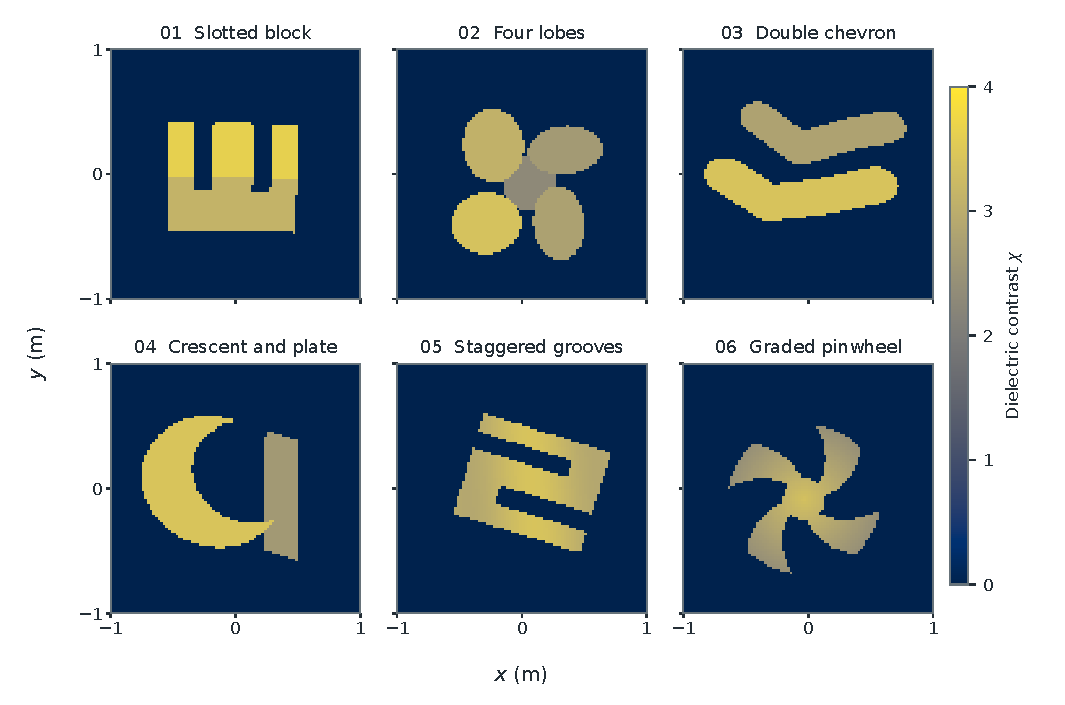
\includegraphics[width=.88\linewidth]{contrast-maps.pdf}
\caption{Reference contrasts on the \(2\,\mathrm{m}\) square, shown on a common scale. Every reported bound for these fields leaves all \(96^2\) contrast values free.}
\label{fig:contrast-maps}
\end{figure}

The reference contrasts in figure~\ref{fig:contrast-maps} have similar peaks and distinct areas and dielectric masses (table~\ref{tab:scattering-statistics}). The Born errors in this table compare the clean nonlinear field \(Y_c\) with the Born field \(Y_{\rm B}\) of the \emph{same} material on the native grid. They range from 4.07 to 6.61 relative to \(\|Y_c\|_F\). The model-wide comparison in section~\ref{sec:exp-inversion} allows the Born material to differ from the reference.

\begin{table}[tbp]
\centering\small
\caption{Native full-ring statistics. Mass is \(\int\chi\,{\rm d}A\), area includes cells with \(\chi>0\), and the Born error is \(\|Y_c-Y_{\rm B}\|_F/\|Y_c\|_F\). The right column uses the same quadrant weights on all six objects. A ratio \(d/r>1\) excludes the nonlinear material box at \(u=0.75\).}
\label{tab:scattering-statistics}
\setlength{\tabcolsep}{4.0pt}
\begin{tabular}{@{}lrrrrrr@{}}
\toprule
Object & \(\max\chi\) & Mass (\(\mathrm{m}^2\)) & Area (\(\mathrm{m}^2\)) & \(\|Y_c\|_F\) & Born error & \(d/r\), 1\%\\
\midrule
01 Slotted block & 3.632 & 2.475 & 0.739 & 4.548 & 6.614 & 2.505\\
02 Four lobes & 3.384 & 2.694 & 0.925 & 5.403 & 5.846 & 0\\
03 Double chevron & 3.416 & 2.553 & 0.811 & 5.409 & 5.715 & 0\\
04 Crescent and plate & 3.437 & 2.359 & 0.748 & 4.786 & 5.908 & 1.061\\
05 Staggered grooves & 3.408 & 2.108 & 0.671 & 4.401 & 5.996 & 1.833\\
06 Graded pinwheel & 3.346 & 1.525 & 0.550 & 5.050 & 4.069 & 0\\
\bottomrule
\end{tabular}
\end{table}

\subsection{Multiple illuminations, negative inertia and single-source bounds}\label{sec:exp-array}

At \(u=0.75\), the maximum over global weights, four-quadrant weights and two fixed sixteen-region weight fields excludes \(3,3,2,0,0\) objects at \(0.5,1,2,5,10\%\) noise, respectively (figure~\ref{fig:exclusion-envelope}(a)). The paired observations follow the original complex 2\% noise direction for each shape, with the 2\% arrays retained verbatim. A separate independent 10\% draw is used in the inversion tests below. Global weights alone pass on \(3,2,2,0,0\) objects, and the fixed sixteen-region fields pass on \(2,2,2,0,0\). The quadrant weights recover the third case, Crescent and plate, at 1\%. A uniform sector weight \(\mu_0=10^{-4}\) with optical weights \((4,16,16,16)\times10^{-6}\) gives \(d\ge0.05077102\) against \(r=0.04786783\). At 2\% this profile gives \(d/r=0.519\) for the same object. At 1\%, the best candidate from 8,987 numerical global proposals gives an upper endpoint of \(0.036671\) for that profile's lower-bound formula.

\begin{figure}[tbp]
\centering
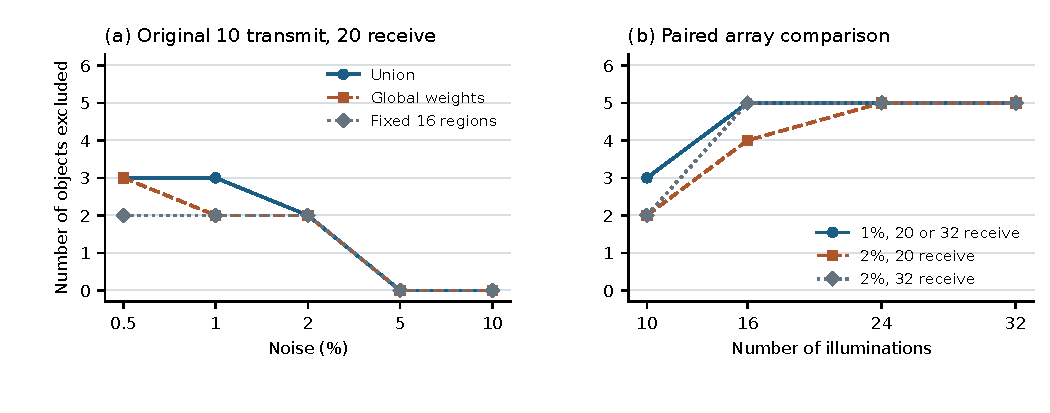
\includegraphics[width=\linewidth]{contrast-exclusions.pdf}
\caption{Excluding the full-wave cap \(u=0.75\) on six objects. (a) At the original full-ring geometry, the union over global, quadrant and fixed sixteen-region weights is nonincreasing with the paired noise level. The quadrant curve coincides with the union. (b) Increasing the number of uniformly distributed plane waves improves exclusions for both tested receiver counts. The four noise and receiver conditions shown are paired on the same materials.}
\label{fig:exclusion-envelope}
\end{figure}

For those fixed quadrant weights, \(K\) is shared by all six objects and has exactly four negative eigenvalues. The fifth eigenvalues of \(H_Y\) at 1\% in object order are \(0.010760,-0.021933,-0.022434,0.002578,0.006506,-0.022918\). Only Slotted block has a positive sixth eigenvalue as well. Four lobes and Double chevron have the largest clean norms and dielectric masses. Their positive source spectrum is exhausted by the four directions removed in Theorem~\ref{th:bound}. The decision is therefore controlled by the remaining coherent responses. For Crescent and plate, the fifth eigenvalue changes by only 4.4\% when the noise doubles, while the squared radius grows fourfold.

\begin{figure}[tbp]
\centering
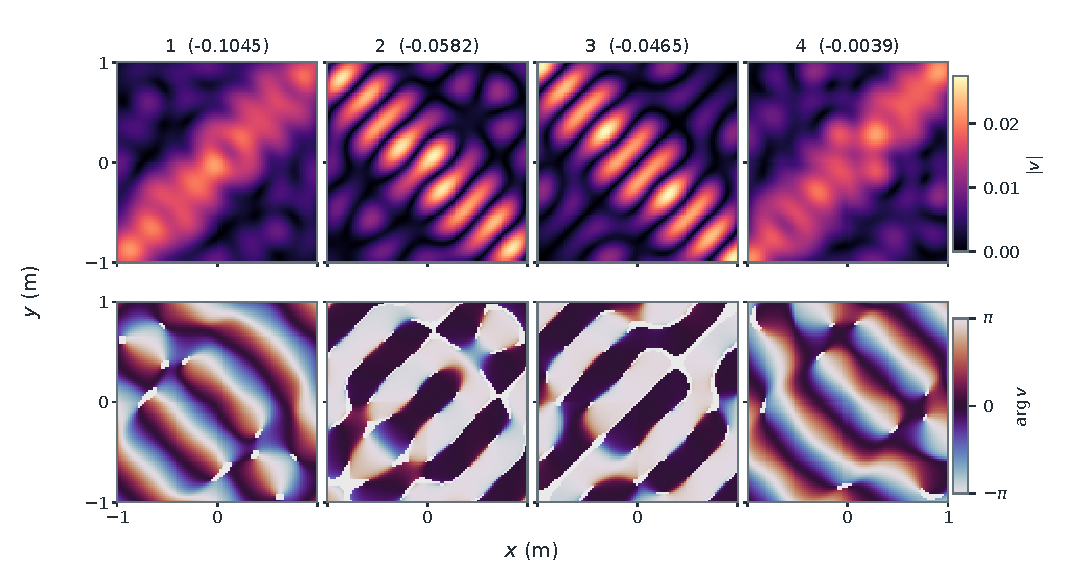
\includegraphics[width=.94\linewidth]{negative-currents.pdf}
\caption{Magnitude (top) and phase (bottom) of the four unit negative eigenvectors of \(K/\mu_0\) for the quadrant weights at \(u=0.75\). Each panel heading gives the mode index and eigenvalue. The phase is set to zero at the largest-amplitude cell and masked below 5\% of that mode's maximum.}
\label{fig:negative-currents}
\end{figure}

These four geometry-dependent directions overlap the poorly observed currents used in subspace-based inversion \cite{chen,zhong}. Each has 99.9931--99.9943\% of its energy in \(\ker S\), yet \(v^*Rv=0.01757\)--\(0.03450\) in the stored Green normalization. A 720-angle quadrature of the outgoing radiation pattern agrees with these powers to \(2\times10^{-15}\). Projection into the receiver kernel leaves almost all of this radiation. The outgoing constitutive residual \(\|(I-0.75G)v\|_2\) is at least \(1.084\) over the whole unit negative span, which is incompatible with a free mode of the uniform cap medium. Actual full-wave reference currents place only 0.23--1.60\% of their energy in this span. A rank-four, receiver-projected Fourier space generated by the nearest four corner frequencies captures 0.06--1.00\% of each mode's dark energy. With 64 Fourier columns the projection captures 99.30--99.36\%, with principal angles of \(3.2^\circ\)--\(5.9^\circ\). Figure~\ref{fig:negative-currents} thus depicts dark directions of the quadratic bound for these weights. A resonance interpretation would require a separate outgoing state test for the material of interest.

For the illumination sweep, \(s=10,16,24,32\) shots have amplitudes \(\sqrt{10/s}\), giving equal total incident fluence in the model. Receiver channels are weighted by \(\sqrt{20/p}\) for \(p=20,32\), including the same change of coordinates in the noise. On \(u=0.75\), the 1\% counts are \(3,5,5,5\) for either receiver count. At 2\%, they are \(2,4,5,5\) for \(p=20\) and \(2,5,5,5\) for \(p=32\). Graded pinwheel remains unresolved throughout. The bandwidth estimate in \eqref{eq:bandwidth} gives \(2ka=23.70\) for the full search square, and the true supports fit in circles with \(2ka=11.89\)--\(14.86\). Angular interpolation from 24 illuminations recovers independently computed clean responses at 32 illuminations with 0.0082--0.1423\% relative error. At 16 illuminations these errors are 2.63--13.42\% (figure~\ref{fig:electrical-scaling}(a)). The simulated responses change little on adding eight angles beyond 24 at the tested tolerances.

The exact negative counts of the bare reactive matrix \(I-u\operatorname{Re}_{H}G\) are \(19,21,25,36,45\) at \(u=0.75,1,1.25,1.5,2\). With fixed weights \(\mu=10^{-4}\) and \(\lambda/\mu=0.1\), the weighted counts are \(4,16,20,22,\ge39\) for 20 receivers and \(4,13,16,20,\ge34\) for 32. For these weights the \(u=2\) sums are empty even with 32 sources. At \(u=1\), 32 sources and 32 receivers at 2\% noise leave seven positive retained eigenvalues with \(d/r=0.3011\) for the strongest replayed scalar choice. At \(u=1.25\) and \(1.5\) those ratios are 0.1133 and 0.01494. Thus \(s>\nu\) can leave too little surviving source response to reach the data threshold. On the smaller annular benchmark, the fixed real-sector choice at \(u=5\) has \(\nu=4\) for 12 shots and gives \(d>0.01469\) with \(r\simeq0.010517\). The experiments resolve a competition between electrical-area growth of reactive directions and the angular bandwidth of the response. The observed thresholds belong to the tested weights and acquisitions.

\begin{figure}[tbp]
\centering
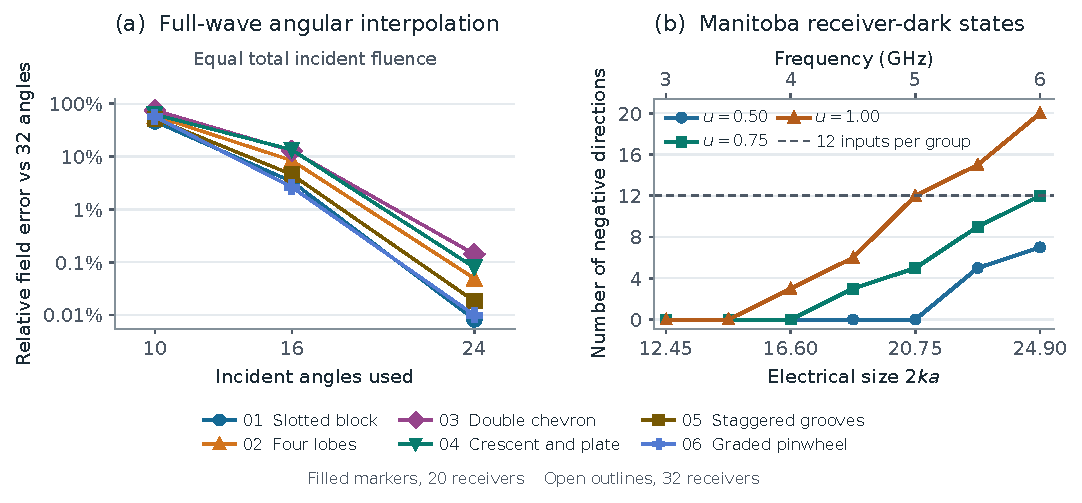
\includegraphics[width=\linewidth]{electrical-scaling.pdf}
\caption{(a) Relative error of interpolated full-wave complex responses against a 32-angle calculation, at equal total incident fluence. The points are paired by material and receiver count. (b) Numerical negative counts of the real-sector state form restricted to the receiver kernel of one Manitoba group. The dashed line marks the 12 incident fields in that group. The full state count also depends on the positive receiver term and is reported in the text.}
\label{fig:electrical-scaling}
\end{figure}

At 2\% noise, Slotted block and Staggered grooves also give a strict comparison with one coherent illumination. The joint constant-weight bounds are \(0.16069878\) and \(0.11060787\), above the respective radii \(0.09096764\) and \(0.08802506\). Theorem~\ref{th:two} gives global single-source exact fits for all unit coherent inputs. In the four-region single-source semidefinite program, receiver-exact first and second moments satisfy the local sector and optical balances and attain zero residual for every such input. Their uniform current energies are below 8,500 and 7,000 in the unweighted native coordinates. A single physical current at the stated cap has energy above 8,886.62, so these moments survive every scalar cap valid for the whole box and every coherent input. They also survive the individual error-ball energy caps \(4.983\times10^6\) and \(1.035\times10^6\). With sixteen regions the best coherent bounds are approximately \(0.18967408\) and \(0.12452151\), excluding both caps. Each resulting positive-definite state matrix leaves only one positive source eigenvalue, making the joint and best coherent values equal for that profile.

\subsection{Microwave chambers and conditional error margins}\label{sec:exp-chambers}

The Manitoba data contain four dielectric objects at seven frequencies from 3 to 6 GHz \cite{manitoba}. Two disjoint parity groups preserve \(288\) of \(552\) directed channels. Calibration uses an empty-chamber reading and a metal cylinder, with a second empty reading and a second cylinder as checks. For the four possible reference combinations, a proved distance at the primary calibration loses at most the largest field displacement to another combination. Subtracting this displacement leaves a positive passive-sector margin on \(20,5,3,1\) of the \(28\) views at caps \(0.25,0.50,0.75,1\), respectively (figure~\ref{fig:cal-headroom}). The E-shaped polyethylene object at 3.5 GHz leaves 1.358\% of the primary norm at cap 0.5, and the large nylon cylinder at 3 GHz leaves 4.018\% at cap 1. If \(\chi=x+\mathrm{i}y\) with \(x>0\), the passive-sector cap concerns \(x+y^2/x\).

\begin{figure}[tbp]
\centering
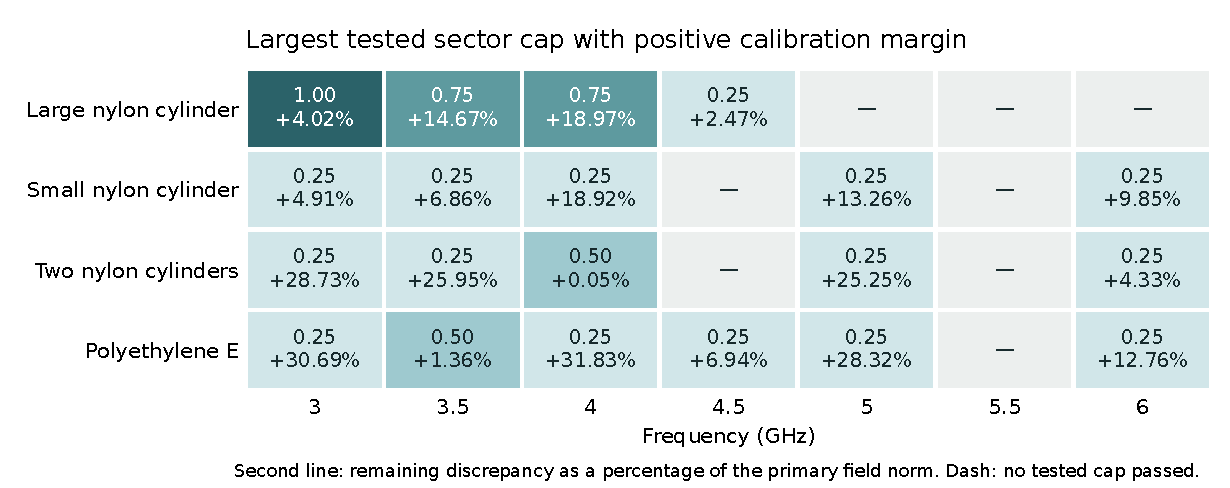
\includegraphics[width=.94\linewidth]{chamber-headroom.pdf}
\caption{Largest tested passive-sector cap with positive remaining distance after allowing any field in the convex hull of four Manitoba calibrations. The second line gives the remaining target-dependent allowance as a percentage of the primary field norm. Each row follows the same object across frequency.}
\label{fig:cal-headroom}
\end{figure}

The fixed \(0.14\,\mathrm m\) square grows from \(1.40\lambda\) to \(2.80\lambda\). At \(u=1\) the real-sector rule \(\mu=\|S\|_2^2/100\) gives full-state negative counts of \(0,0,3,8,12,15,20\) across the seven frequencies in the evaluated parity group. Restricting to \(\ker S\) gives \(0,0,3,6,12,15,20\), as in figure~\ref{fig:electrical-scaling}(b). At 5 GHz and above this choice leaves no source direction in that 12-shot group. Individual conditional margins still depend on calibration and target. The polyethylene target recovers a positive margin at 6 GHz after losing it at 5.5 GHz.

For Fresnel, we use the measured total-minus-incident fields at 4, 6 and 8 GHz, the fitted empty-field incidence and 241 receiver angles per shot \cite{fresnel}. The two individual cylinder arrangements have eight illuminations and the twin arrangement has eighteen. No tested field rules out \(u=0.5\) under the held-out empty-scene scale. At 4 GHz and \(u=0.25\), the twin arrangement's real-sector bound is 28.515\% of \(\|Y\|_F\). Inserting an additive scale of 8.884\% and a gain scale of 10.41\% into \eqref{eq:budget} leaves 6.98\% for further discrepancy. Nominal full-wave calculations with 60 and 120 cells per side differ in their full port predictions by 0.79--5.73\% across the nine views. Their residuals also include target and instrument mismatch, so these grid differences do not enclose the error of the chamber model.

The fixed-port test of the unrestricted nonnegative Born model in \eqref{eq:born} uses the actual receiver masks. In Manitoba two calibration comparisons are the difference between metal references and the empty drift plus held-out metal residual. The Born lower distances are 28.16--88.30\% of the selected field norm and exceed both scales on 25 of 28 views. In Fresnel the three lower bounds at 4 GHz are 38.36--44.85\%, above the transferred empty-field RMS scale both with and without the diagnostic complex-gain allowance. None of the six higher-frequency views exceeds both scales. These comparisons are conditional on the chosen calibration budget and the real, nonnegative Born class. Loss, antenna and three-dimensional modeling can contribute to the measured discrepancy. The experiments do not bound their combined effect on unknown loaded targets.

\subsection{Use before and during inversion}\label{sec:exp-inversion}

On the main full-ring data, the nonlinear bound rules out \(u=0.5\) for all six materials at 1\%, 2\% and independent 10\% noise. Its lower distance is 6.62--13.57 times the radius at 2\%, and 1.32--2.71 times the radius at 10\%. This calculation uses the data before any iterative inversion. Separately, the fixed finite-port test in \eqref{eq:born} rules out every nonnegative first-Born image for all 96 paired strong-scattering views in the array sweep. Its lower distances are 40.23--61.56\% of \(\|Y\|_F\). It requires one geometry-dependent weight per array. For a weak full-wave ellipse and a deliberately Born-generated control, explicit Born predictions lie in the noise balls. For full-wave paired disks with peak 0.04, the fixed weight yields zero. Selecting a direction from the data gives lower distances of \(5.348r\) and \(2.748r\) at 1\% and 2\% without restricting the Born contrast amplitude. The cheap fixed readout is consequently sufficient for these strong cases and can miss a departure from Born at small contrast. The two checks address different model classes.

\begin{table}[tbp]
\centering\small
\caption{Measured wall times, separating reusable setup from one new data matrix. The timings include numerical proposals and interval checks as stated.}
\label{tab:cost}
\begin{tabular}{@{}>{\raggedright\arraybackslash}p{.28\linewidth}
                 >{\raggedright\arraybackslash}p{.39\linewidth}
                 >{\raggedright\arraybackslash}p{.23\linewidth}@{}}
\toprule
Test & Setup or cold computation & Per new reading after setup\\
\midrule
Fixed port weighting, \(96^2\) & \(0.2\)--\(0.8\,{\rm s}\) per array & about \(0.5\,{\rm ms}\)\\
Full-wave cap test, \(96^2\) & \(57.54\,{\rm s}\) for stationary responses, \(3.84\,{\rm s}\) for negative gaps & \(5.89\,{\rm ms}\) median for six profiles\\
Initial state checks, \(96^2\) & \(1.33\)--\(34.75\,{\rm s}\) per profile & --\\
Full-wave cap test, \(12^2\) & \(0.70\)--\(0.74\,{\rm s}\) cold per reading & --\\
\bottomrule
\end{tabular}
\end{table}

Among the six large scatterers, the lower bound itself rules out a fit within \(2.5r\) for 15 of the 23 excluded object--noise--cap conditions. In the eight remaining eligible conditions, zero-start, penalized full-wave fits retained residuals above \(2.5r\) after up to 94 objective calls. An ordinary residual check would already reject those reconstructions. We therefore tested the intervention on a separately designed compact patch with peak 0.879, mean 0.654 and side \(\lambda/6\). The clean field difference to the uniform \(0.5\) square sets the scale for four fixed relative noise levels of \(12.38\)--\(26.13\%\). These are repeated measurements of one constructed material. Every method sees the same physical forward map, data and radius. It starts at zero with the same spatial penalty and the same budget. The low-cap algorithm converges to the uniform \(0.5\) square in six calls, achieving residuals of \(1.487\)--\(2.481r\), within a lenient \(2.5r\) stopping threshold. The full-box lower bound is \(1.437\)--\(2.422r\), so all configurations below that cap miss the stipulated noise ball.

Broad release to cap 2 gives residuals of \(0.991\)--\(0.992r\) and reduces separately simulated held-out complex field error from 27.50\% to 1.32--2.52\%. The relative material error rises from 0.462 to \(0.721\)--\(0.943\), and the peak rises to 1.85--2.00. At the same six-call checkpoint as the low-cap run, the released path has relative material error \(0.315\)--\(0.317\), but only one reading falls inside \(r\). A rule using the exact point discrepancy releases the cap for all four views and reaches nearly the same final errors as immediate broad release. Accordingly the class-wide test can change a decision under lenient stopping, while a stringent residual check recovers almost the same broad-release outcome.

\begin{figure}[tbp]
\centering
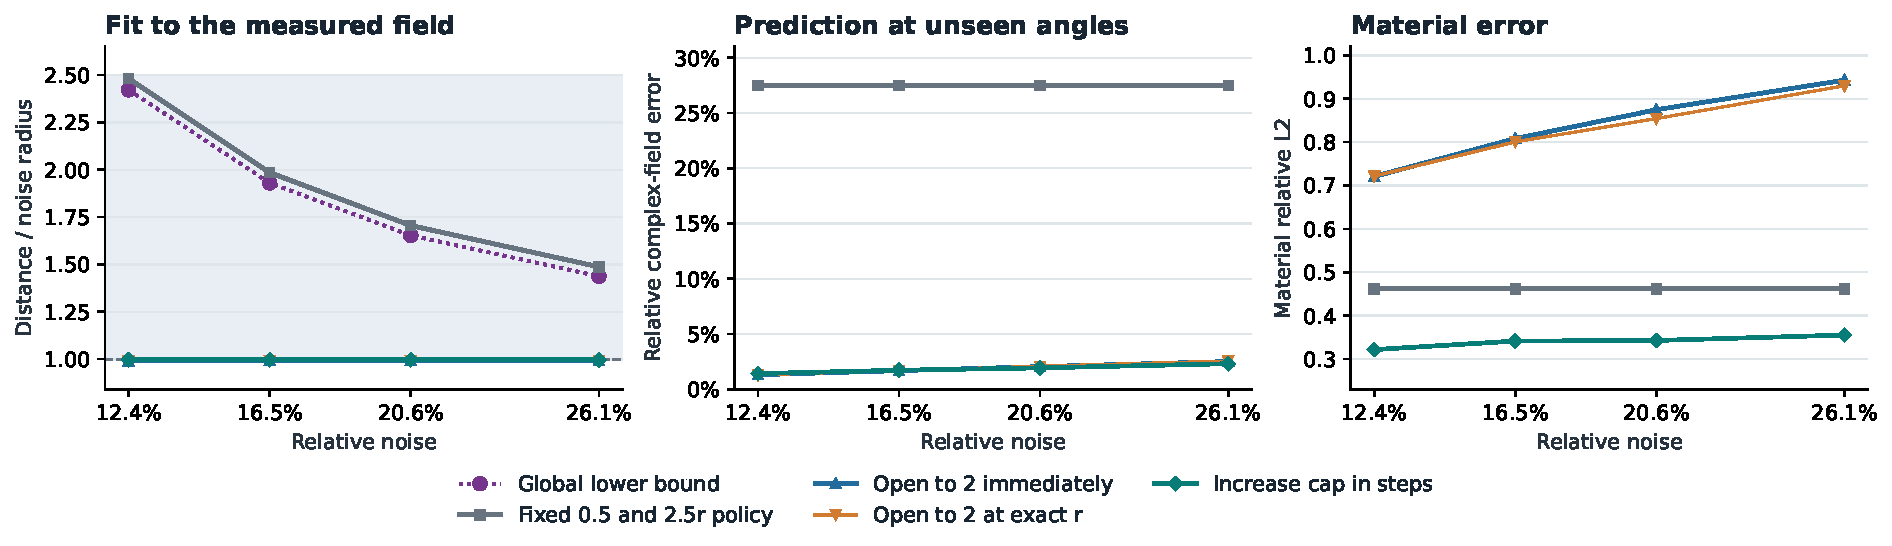
\includegraphics[width=\linewidth]{inversion-tradeoffs.pdf}
\caption{One compact object under four error levels. The lenient residual rule accepts the low-cap shape although the lower bound for the entire cap lies above the error radius. Immediate broad release improves prediction at unseen angles and worsens the final material error. Incremental release limits the excess peak.}
\label{fig:inversion-tradeoff}
\end{figure}

On the same exposed compact object we also compared incremental cap release at \(0.5,0.6,0.75,1,1.25,2\), with the same warm-start rule, material grid and point discrepancy test. Using the class result skips the infeasible first cap. Both policies first enter the ball at 0.75 and produce bitwise identical maps, with material relative errors of \(0.322\)--\(0.355\), interior errors of \(0.170\)--\(0.175\) and held-out field errors of 1.42--2.32\%. Guidance reduces objective calls from 22 to 19. Charging the cold class test in table~\ref{tab:cost} erases that time saving on the compact grid. This example establishes a class decision and a possible reduction in search work with reusable setup. The tested continuation already obtains the same reconstruction quality.

\FloatBarrier


\section{Discussion}\label{sec:discuss}

\subsection{Which material information reaches the receivers?}
Peak contrast and angular resolution enter in different places. Increasing the trial cap makes it easier for unobserved currents to offset the sector bound. Adding independent incident fields can expose the shared material through cross-illumination terms. Additional shots achieve little once the incident field on the active scatterer, propagated to the receivers, is well interpolated from the shots already used. The $2ka$ scale describes that angular dependence. It fixes neither the index of a particular weighted current matrix nor the last positive eigenvalue of the measured source form. In the six-object test, both mechanisms can be observed on the same physical grid. The drop in the distance at larger contrast persists on a ring with 32 receivers and 32 illuminations.

The negative eigenvectors reveal another distinction. A current can be nearly invisible at the receivers and still have a large defect in the homogeneous outgoing equation for a proposed uniform material. Only a small fraction of the reference currents in the six heterogeneous objects lies in the four negative directions studied here. Inserting these four vectors as putative resonant modes of a reconstruction would require separate evidence of overlap with the material-induced currents. Their directly established role is to limit the measured illumination spectrum available to a contrast bound.

Even a valid peak statement can carry little spatial information. For a tested region $A$ and fixed exterior weights, the quadratic restricted to currents in $A^c$ is completely independent of the multipliers inside $A$. The min--max principle gives $\nu\ge n_-(K_{A^c,A^c})$. When this exterior count reaches $s$, \eqref{eq:bound} vanishes for all choices of the interior weights. On the spatial tests in the appendix, this explains why a positive global lower bound could coexist with no localized lower peaks. Likewise, stacking two frequencies can incur a joint index penalty while separate frequency bounds retain positive terms. Neither the frequency nor the geometry of a receiver by itself orders the information content of two measured fields.

\subsection{What a reconstruction can use}
A bounded-error inverse can also be studied by following nonlinear solution branches \cite{everett96,everett26,vasco} or subdividing parameter space \cite{sivia}. Strong localized scatterer reconstructions use location and sparsity assumptions \cite{chai}, and interaction-matrix completion imposes consistency with the scattering operator \cite{levinson}. Finite-measurement uniqueness results impose explicit restrictions on coefficients or on the class of scatterers \cite{alberti19,alberti21,kuo_novikov}. The peak bound instead applies to every arrangement in the stated cell box, including objects with unknown support. It need not identify a branch or a spatial image. A null space at a finite receiver array is also compatible with radiated fields elsewhere. Transmission eigenvalues and non-scattering waves concern a different condition on the whole exterior field \cite{cakoni_book,cakoni_vogelius}.

For a method that updates the contrast and current together \cite{csi}, or that changes the integral equation to handle stronger scattering \cite{nie,cie}, there are two immediate data decisions. A positive Born distance above $r$ rules out using the linear model with any nonnegative image. A positive full-wave distance above $r$ rules out retaining the proposed contrast range even with a nonlinear solver. The compact example shows why further guidance is needed to recover an image. A gradual increase in permissible contrast improved the material fit. A small full-wave residual alone drove the unconstrained range beyond the true peak. Ordinary discrepancy continuation obtained exactly the same final image as the bound-guided continuation. In this experiment the additional result is global information about the discarded class. We found no improvement in reconstruction over an equally informed stopping rule.

\subsection{Physical range of the result}
In the computations, strict peak inequalities apply to the full stated discrete scalar model and a noise ball containing the synthetic generator. Coarser and finer fields for the same material can differ by tens of per cent. A waveguide or microwave chamber also introduces antenna coupling, calibration, loss and out-of-plane structure. In particular the two empirical calibration comparisons in the Manitoba experiment do not provide an upper bound on the model discrepancy of a loaded target. Reporting the remaining margin gives a physical criterion against which an independently measured uncertainty could be compared. Extending the bounds to a continuous dielectric or a three-dimensional tensor material requires control of the corresponding forward error and the appropriate local constitutive law.

\subsection*{Data and code availability}
The accompanying numerical material contains the synthetic port fields, hypotheses, lower distances, angular interpolation errors, current and source spectra, and inputs for the figures. It records flat and inconclusive outcomes. The measured fields are available from the Institut Fresnel and University of Manitoba repositories described in \cite{fresnel,manitoba}. The numerical material documents their masks, calibration procedures and derived margins.

\section*{Acknowledgements}
\paragraph{Use of generative AI.} OpenAI Codex and Google Gemini assisted with mathematical development, scientific programming, comparison with the literature and preparation of the manuscript. Section~\ref{sec:fourier} specifies their roles in the numerical work. Forward residuals, spectral margins and measured-data comparisons were checked against the stored physical operators as described in Appendix~\ref{app:replay}. The authors take responsibility for the analysis, the interpretation and the manuscript.

\appendix
\section{Numerical bounds and uncertainty}\label{app:replay}

\paragraph{Retained Fourier modes.}
For regional weights in \eqref{eq:floor}, put $w_i=(D_\mu)_{ii}/\mu$, $t_i=(D_\lambda)_{ii}/\mu$ and $z_i=\{u(w_i-1)+\mathrm i(t_i-t)\}/2$. The cross term couples $V_Fj$ with $V_F\diag(\bar z_i)j$. For a real $c$ and $\beta>0$, each omitted two-variable form is positive semidefinite when $\sigma_q-f\ge |g_q-c|^2/\beta$. Summing gives the cellwise floor $f+w_i-1-2c\Re z_i-\beta|z_i|^2$, with signed updates of rank at most two per retained mode. The compact constant-weight system had order at most 645. Both nonuniform sixteen-region systems had order 1,478.

\paragraph{Native stationary defect.}
The $192^2$ padded symbol gives the full-grid defect $\Delta$ in \eqref{eq:native}. With $g$ a positive spectral floor, we subtract $\mu\norm{\Delta}_F^2/g$ from the trial source form to bound $H_Y$ in \eqref{eq:operators}. The shifted Fourier form bounds the negative index above and a native negative subspace bounds it below. Complex ball arithmetic encloses the resulting source Rayleigh quotients \cite{arb}. Theorem~\ref{th:bound} applies when the outward lower endpoint exceeds the radius. An absolute spectral gap also permits an upper endpoint for a given weight profile.

\paragraph{Error radii.}
We use the deterministic radius $r=\delta+10^{-6}\norm{Y}_F$. The sampled norm $\delta$ alone missed 16 of 24 reference fields by up to $1.87\times10^{-11}$ field units. The pad covers numerical generation error for all 24 fields and all 30 paired full-ring views. For the same materials, the coarse and fine fields differ by 12.4--28.4\% in half aperture and 14.2--35.4\% in full aperture. Grid and chamber transfers require a separate uncertainty term in \eqref{eq:budget}.

\paragraph{Energy-constrained four-region moments.}
For $K-\tau I\succ0$, completing \eqref{eq:completion} gives $\norm{Sj-Ya}^2\ge\tau\norm{j}^2+a^*H_\tau a$, where $H_\tau=Y^*Y-L^*(K-\tau I)^{-1}L$. If $\lambda_{\min}(H_\tau)\ge\ell_\tau$, then $\norm{j}^2\le (r^2-\ell_\tau)/\tau$ for every coherent input in its error ball. To bound the energy without data, 64 plane-wave columns give $S^*S\preceq\gamma R+\eta I$, with $\gamma=1/128$ and $\eta<5.14\times10^{-10}$. The floor $K/\mu\succeq(3/256)I$ gives $K_{\rm pow}=K-S^*S+\gamma R\succ0$. A second completion at $K_{\rm pow}-\tau I$, with coefficient $(Z+\mathrm i\gamma I/2)B$, bounds the energy by $2{,}340{,}476$ throughout the box. The separate error-ball caps are $4{,}982{,}633$ and $1{,}035{,}001$.

For the two full-ring 2\% examples at $u=0.75$, eight receiver-null directions and a receiver-exact mean satisfy \eqref{eq:regionalmoment}. The lifted moments have rank at most nine and their current traces are below $8{,}500$ and $7{,}000$ uniformly over unit input. A physical material in the box attains energy above $8{,}886.62$ for a fixed unit input. Thus the four-region optimum is exactly zero under every uniform energy cap valid on the box and under the stated separate caps. For the artificial cap 100, the receiver-only lower distances are 0.9730 and 1.0280. The energy where the four-region optimum first becomes positive is open.

Theorem~\ref{th:two} yields a simultaneous coherent fit and strict lifted feasibility on 25 of 30 paired views, including every view excluded at $u=0.75$. The other five 10\% views remain undecided by that construction. At the sixteen-region weights each of the two 2\% examples has one positive source eigenvalue. The leading coherent direction therefore gives the full fixed-weight distance in \eqref{eq:bound}.

\begin{table}[!tb]
\centering\footnotesize
\setlength{\tabcolsep}{4pt}
\caption{Replay and comparison costs on Apple M4. Times are wall and process CPU seconds. Dashes denote an unavailable or nonadditive timing. The first global and four-region $u=0.75$ batches each include 45 inconclusive evaluations. Refinement of the 15 affected views is charged separately.}
\label{tab:replay}
\begin{tabular}{@{}>{\raggedright\arraybackslash}p{.39\linewidth}
 >{\raggedleft\arraybackslash}p{.145\linewidth}
 >{\raggedleft\arraybackslash}p{.145\linewidth}
 >{\raggedright\arraybackslash}p{.24\linewidth}@{}}
\toprule
Calculation & Wall & CPU & Scope\\ \midrule
Paired full-ring proposal search & 12.79 & 12.73 & Shared across five caps\\
Constant weights, $u=0.50$ & 49.52 & 49.97 & Native replay\\
Constant weights, $u=0.75$ & 213.88 & 211.86 & First batch\\
Constant-weight refinement & 20.20 & 19.98 & 15 views\\
Four regions, $u=0.75$ & 316.14 & 312.89 & First batch\\
Four-region refinement & 42.40 & 42.50 & 15 views\\
Sixteen-region symmetric search & 66.29 & --- & 84 trials, one case missed\\
Nonuniform search and native ranking & 22.49 & --- & Both cases\\
Sixteen-region coherent proof & 69.44 & --- & Both cases\\
Joint reuse & 6.09 & --- & Existing state proofs\\
30-view cross-application & 20.50 & 21.36 & Existing state proofs\\
Three higher caps, same fixed profiles & 14.59 & 14.88 & Native checks\\
Crescent and plate, dense scalar control & 59.53 & 58.62 & Search included\\
Energy caps, gap and error-ball proofs & 283.57 & 509.99 & Both cases, concurrent work\\
Energy-capped moments & 10.58 & 10.55 & Final construction and proof\\
Energy-capped moments, exploratory subtotal & --- & 54.42 & Measured costs including final path\\
Regional localization, $U_{\max}=20$ & 12.6/51.7 & 12.4/48.7 & Search and interval check\\
Regional localization, $U_{\max}=4$ & 162.8/152.2 & 154.9/136.8 & Search and interval check\\
Two-frequency comparison & 17.05/40.95 & 16.36/40.34 & Search and positive-point checks\\
Fixed profiles, 22-object transfer & 63.20 & 67.10 & Shared responses included\\
\bottomrule
\end{tabular}
\end{table}

The nonuniform path cost 91.93~s or 158.22~s including the symmetric trials. The full-box energy proof adds 4.30~s after the gap proof and the independent physical current check adds 1.19~s. The 54.42~s CPU subtotal includes rejected numerical proposals with receiver leakage. Ten other exploratory records lack separate timings. One rejected interval check had already applied the Green operator to four dark and ten fitted columns. High-cap subspace proposals and their outward evaluation took 8.64 and 6.50~s, respectively.

\section{Regional, frequency and transfer controls}\label{app:controls}

\paragraph{Regional localization.}
Six $32^2$ materials contributed seven views and sixteen regions per view. At both exterior caps $U_{\max}=20$ and $4$, the result was 0/112 for excluding an empty region and 0/112 for a positive local peak lower bound. The exterior principal block alone has at least 116 and 106 negative directions at $U_{\max}=20$ for the twenty- and ten-source layouts, and at least 24 and 14 at $U_{\max}=4$. The result holds over $0\le\lambda/\mu\le128$ and for sector scales at least their tested minimum, irrespective of interior weights. Each search used 192 base $LDL^*$ factorizations. The tighter box reused 76 inverses in 27,904 compact updates before interval checks.

\paragraph{Two frequencies.}
The same six nondispersive materials and half ring were used at 400 and 500 MHz. Weights may mix frequency components at a pixel because $I_2\otimes X$ repeats the material there. At cap 0.50 and 2\% noise, independent frequency distances in quadrature exceeded the nominal radius in 3/6 cases. Mixed weights gave 0/6, and both approaches gave 0/6 at 10\%. Adding each coarse reference discrepancy gave 0/6 under both approaches at both noise levels. Separate treatment pays the negative-index penalty per frequency. The screen used 32 factorizations of order 1,024 and 33 of order 2,048. The three positive points were checked separately on the inverse grid.

\paragraph{Transfer.}
Unchanged profiles gave 22/22 joint and 20/22 coherent exclusions of cap 0.50 on additional full-ring $96^2$ materials at 10\% noise. Both gave 0/22 at cap 0.75. Across the 110 latter profile evaluations, the largest upper endpoint was $0.1682r$. On the separate $24^2$ ring with 12 inputs, 48 receivers and 1\% noise, the fixed real-sector profile had four negative directions. The joint result at cap 5 was 5/7, at distance ratios 5.12--10.77, versus 0/7 with the tested coherent profiles. One undecided material had peak 16.25. The other had peak 4.28, supplying a feasible medium under cap 5. The reference media for both acquisitions satisfied their respective padded or original error balls.

\paragraph{Measured-channel controls.}
For three Fresnel targets at 4, 6 and 8 GHz, source groups use common measured rows among the 241 valid receivers per source \cite{fresnel}. At cap 0.50 none of nine views exceeded its held-out empirical calibration scale. In Manitoba the antisymmetric field component is 0.62--5.98\% of the primary norm. Projecting all four calibrations onto their reciprocal parts preserved the same positive-margin views. The loaded-scene discrepancy in \eqref{eq:budget} remains unknown.

\FloatBarrier

\FloatBarrier
\begingroup\small
\begin{thebibliography}{99}\setlength{\itemsep}{0pt}\setlength{\parsep}{0pt}
\bibitem{chen} Chen X 2010 Subspace-based optimization method for solving inverse-scattering problems \emph{IEEE Trans. Geosci. Remote Sens.} \href{https://doi.org/10.1109/TGRS.2009.2025122}{\textbf{48} 42--49}
\bibitem{zhong} Zhong Y and Chen X 2009 Twofold subspace-based optimization method for solving inverse scattering problems \emph{Inverse Problems} \href{https://doi.org/10.1088/0266-5611/25/8/085003}{\textbf{25} 085003}
\bibitem{ffttsom} Zhong Y and Chen X 2011 An FFT twofold subspace-based optimization method for solving electromagnetic inverse scattering problems \emph{IEEE Trans. Antennas Propag.} \href{https://doi.org/10.1109/TAP.2010.2103027}{\textbf{59} 914--927}
\bibitem{angeris19} Angeris G, Vu\v{c}kovi\'{c} J and Boyd S P 2019 Computational bounds for photonic design \emph{ACS Photonics} \href{https://doi.org/10.1021/acsphotonics.9b00154}{\textbf{6} 1232--1239}
\bibitem{trivedi} Trivedi R, Angeris G, Su L, Boyd S, Fan S and Vu\v{c}kovi\'{c} J 2020 Bounds for scattering from absorptionless electromagnetic structures \emph{Phys. Rev. Applied} \href{https://doi.org/10.1103/PhysRevApplied.14.014025}{\textbf{14} 014025}
\bibitem{angeris} Angeris G, Vu\v{c}kovi\'{c} J and Boyd S 2021 Heuristic methods and performance bounds for photonic design \emph{Opt. Express} \href{https://doi.org/10.1364/OE.415052}{\textbf{29} 2827--2854}
\bibitem{moleskyglobal} Molesky S, Chao P, Jin W and Rodriguez A W 2020 Global $\mathbb{T}$ operator bounds on electromagnetic scattering: upper bounds on far-field cross sections \emph{Phys. Rev. Research} \href{https://doi.org/10.1103/PhysRevResearch.2.033172}{\textbf{2} 033172}
\bibitem{moleskylocal} Molesky S, Chao P and Rodriguez A W 2020 Hierarchical mean-field $\mathbb{T}$ operator bounds on electromagnetic scattering: upper bounds on near-field radiative Purcell enhancement \emph{Phys. Rev. Research} \href{https://doi.org/10.1103/PhysRevResearch.2.043398}{\textbf{2} 043398}
\bibitem{kuang} Kuang Z and Miller O D 2020 Computational bounds to light--matter interactions via local conservation laws \emph{Phys. Rev. Lett.} \href{https://doi.org/10.1103/PhysRevLett.125.263607}{\textbf{125} 263607}
\bibitem{shim} Shim H, Kuang Z, Lin Z and Miller O D 2024 Fundamental limits to multi-functional and tunable nanophotonic response \emph{Nanophotonics} \href{https://doi.org/10.1515/nanoph-2023-0630}{\textbf{13} 2107--2116}
\bibitem{tian} Tian Y 2013 Closed-form formulas for calculating the extremal ranks and inertias of a quadratic matrix-valued function and their applications \href{https://arxiv.org/abs/1301.2567v1}{arXiv:1301.2567v1}, Corollary~4.5, equation~(4.38)
\bibitem{griesmaier_harrach}
Griesmaier R and Harrach B 2018 Monotonicity in inverse medium scattering on unbounded domains \emph{SIAM J. Appl. Math.} \href{https://doi.org/10.1137/18M1171679}{\textbf{78} 2533--57}
\bibitem{griesmaier_harrach_erratum}
Griesmaier R and Harrach B 2021 Erratum: monotonicity in inverse medium scattering on unbounded domains \emph{SIAM J. Appl. Math.} \href{https://doi.org/10.1137/21M1399221}{\textbf{81} 1332--37}
\bibitem{albicker} Albicker A and Griesmaier R 2023 Monotonicity in inverse scattering for Maxwell's equations \emph{Inverse Probl. Imaging} \href{https://doi.org/10.3934/ipi.2022032}{\textbf{17} 68--105}
\bibitem{bucci87} Bucci O M and Franceschetti G 1987 On the spatial bandwidth of scattered fields \emph{IEEE Trans. Antennas Propag.} \href{https://doi.org/10.1109/TAP.1987.1144024}{\textbf{35} 1445--1455}
\bibitem{bucci89} Bucci O M and Franceschetti G 1989 On the degrees of freedom of scattered fields \emph{IEEE Trans. Antennas Propag.} \href{https://doi.org/10.1109/8.29386}{\textbf{37} 918--926}
\bibitem{colton} Colton D and Kress R 2019 \emph{Inverse Acoustic and Electromagnetic Scattering Theory} 4th edn (Cham: Springer) \href{https://doi.org/10.1007/978-3-030-30351-8}{doi:10.1007/978-3-030-30351-8}
\bibitem{chenbook} Chen X 2018 \emph{Computational Methods for Electromagnetic Inverse Scattering} (Singapore: Wiley) \href{https://doi.org/10.1002/9781119311997}{doi:10.1002/9781119311997}
\bibitem{richmond} Richmond J H 1965 Scattering by a dielectric cylinder of arbitrary cross section shape \emph{IEEE Trans. Antennas Propag.} \href{https://doi.org/10.1109/TAP.1965.1138427}{\textbf{13} 334--341}
\bibitem{boyd} Boyd S and Vandenberghe L 2004 \emph{Convex Optimization} (Cambridge: Cambridge University Press) \href{https://doi.org/10.1017/CBO9780511804441}{doi:10.1017/CBO9780511804441}
\bibitem{beck} Beck A and Eldar Y C 2006 Strong duality in nonconvex quadratic optimization with two quadratic constraints \emph{SIAM J. Optim.} \href{https://doi.org/10.1137/050644471}{\textbf{17} 844--860}
\bibitem{manitoba} Gilmore C, Zakaria A, Mojabi P, Ostadrahimi M, Pistorius S and Lo Vetri J 2011 The University of Manitoba microwave imaging repository: a two-dimensional microwave scattering database for testing inversion and calibration algorithms \emph{IEEE Antennas Propag. Mag.} \href{https://doi.org/10.1109/MAP.2011.6138442}{\textbf{53} 126--133}
\bibitem{fresnel} Geffrin J-M, Sabouroux P and Eyraud C 2005 Free space experimental scattering database continuation: experimental set-up and measurement precision \emph{Inverse Problems} \href{https://doi.org/10.1088/0266-5611/21/6/S09}{\textbf{21} S117--S130}
\bibitem{everett96}
Everett M E 1996 Homotopy, polynomial equations, gross boundary data, and small Helmholtz systems \emph{J. Comput. Phys.} \href{https://doi.org/10.1006/jcph.1996.0070}{\textbf{124} 431--41}
\bibitem{everett26}
Everett M E 2026 Multiple solutions to geophysical inverse problems via tracking flights across a deeply incised model landscape \emph{Geophys. J. Int.} \href{https://doi.org/10.1093/gji/ggag432}{\textbf{247} ggag432}
\bibitem{vasco}
Vasco D W 2000 An algebraic formulation of geophysical inverse problems \emph{Geophys. J. Int.} \href{https://doi.org/10.1046/j.1365-246x.2000.00188.x}{\textbf{142} 970--90}
\bibitem{sivia}
Jaulin L and Walter E 1993 Set inversion via interval analysis for nonlinear bounded-error estimation \emph{Automatica} \href{https://doi.org/10.1016/0005-1098(93)90106-4}{\textbf{29} 1053--64}
\bibitem{chai}
Chai A, Moscoso M and Papanicolaou G 2014 Imaging strong localized scatterers with sparsity promoting optimization \emph{SIAM J. Imaging Sci.} \href{https://doi.org/10.1137/130943200}{\textbf{7} 1358--87}
\bibitem{levinson}
Levinson H W and Markel V A 2016 Solution of the nonlinear inverse scattering problem by \(T\)-matrix completion. I. Theory \emph{Phys. Rev. E} \href{https://doi.org/10.1103/PhysRevE.94.043317}{\textbf{94} 043317}
\bibitem{alberti19}
Alberti G S and Santacesaria M 2019 Calder\'on's inverse problem with a finite number of measurements \emph{Forum Math. Sigma} \href{https://doi.org/10.1017/fms.2019.31}{\textbf{7} e35}
\bibitem{alberti21}
Alberti G S and Santacesaria M 2022 Infinite-dimensional inverse problems with finite measurements \emph{Arch. Ration. Mech. Anal.} \href{https://doi.org/10.1007/s00205-021-01718-4}{\textbf{243} 1--31}
\bibitem{kuo_novikov}
Kuo P C and Novikov R G 2025 Inverse scattering for the multipoint potentials of Bethe--Peierls--Thomas--Fermi type \emph{Inverse Problems} \href{https://doi.org/10.1088/1361-6420/ade282}{\textbf{41} 065021}
\bibitem{cakoni_book}
Cakoni F, Colton D and Haddar H 2023 \emph{Inverse Scattering Theory and Transmission Eigenvalues} 2nd edn, CBMS-NSF Regional Conference Series in Applied Mathematics vol 98 (Philadelphia, PA: SIAM) \href{https://doi.org/10.1137/1.9781611977424}{doi:10.1137/1.9781611977424}
\bibitem{cakoni_vogelius}
Cakoni F and Vogelius M S 2023 Singularities almost always scatter: regularity results for non-scattering inhomogeneities \emph{Commun. Pure Appl. Math.} \href{https://doi.org/10.1002/cpa.22117}{\textbf{76} 4022--47}
\bibitem{csi} van den Berg P M and Kleinman R E 1997 A contrast source inversion method \emph{Inverse Problems} \href{https://doi.org/10.1088/0266-5611/13/6/013}{\textbf{13} 1607--1620}
\bibitem{nie} Zhong Y, Lambert M, Lesselier D and Chen X 2016 A new integral equation method to solve highly nonlinear inverse scattering problems \emph{IEEE Trans. Antennas Propag.} \href{https://doi.org/10.1109/TAP.2016.2535492}{\textbf{64} 1788--1799}
\bibitem{cie} Zhong Y and Xu K 2019 Contraction integral equation for three-dimensional electromagnetic inverse scattering problems \emph{J. Imaging} \href{https://doi.org/10.3390/jimaging5020027}{\textbf{5} 27}
\bibitem{arb} Johansson F 2017 Arb: efficient arbitrary-precision midpoint-radius interval arithmetic \emph{IEEE Trans. Comput.} \href{https://doi.org/10.1109/TC.2017.2690633}{\textbf{66} 1281--1292}
\end{thebibliography}

\endgroup
\end{document}
